%%%%%%%%%%%%%%%%%%%%%%%%%%%%%%%%%%%%%%%%%%%%%%%%%%%%%%%%%%%%%%%%%%%%%%%%%%%%%%%%%%%%%%%%%%%%%
%%									section.	2.	Optimisation combinatoire											%
%%%%%%%%%%%%%%%%%%%%%%%%%%%%%%%%%%%%%%%%%%%%%%%%%%%%%%%%%%%%%%%%%%%%%%%%%%%%%%%%%%%%%%%%%%%%%

\section{Optimisation combinatoire}
	L'optimisation combinatoire, appelée  aussi optimisation discrète, est une branche de l'optimisation en mathématiques appliquées et en informatique, également liée à la recherche opérationnelle, l'algorithmique et la théorie de la complexité, elle consiste à trouver un \emph{meilleur} choix parmi un ensemble fini (souvent très grand) de possibilités. Elle recouvre les méthodes qui servent à déterminer l'optimum ou montrer la difficulté de résoudre une fonction sous des contraintes données, contrairement aux fonctions sans contrainte la solution optimale correspond au coût optimal (minimal, maximal) de la fonction.

	La plupart des problèmes d'optimisation appartiennent à la classe des problèmes NP-difficile classe où il n'existe pas d'algorithme qui fournit la solution optimale en temps polynomial en fonction de la taille du problème et le nombre d'objectifs à optimiser. D'où la nécessité d'utiliser les méthodes approchées (Méta heuristique, Heuristique, etc.) pour obtenir l'ensemble des solutions admissibles aux problèmes.
 Dans ce qui suit nous présentons les concepts et vocabulaires liés au domaine.


\begin{definition}[Fonction objectif]
	Une fonction objectif est une fonction qui modélise le but à atteindre dans le problème d'optimisation sur l'ensemble des critères. Il s'agit de la fonction qui doit être optimisée. Elle est notée $F(x)$ de manière générale $F(x)$ est un vecteur :
$F(x)= [f_1(x), f_2(x),..., f_k(x)]$. Elle est aussi appelée : critère d'optimisation, fonction coût, fonction d'adaptation, ou encore performance.
\end{definition}

\begin{definition}[Paramètres]
	Un paramètre du problème d'optimisation, est une variable qui exprime une donnée quantitative ou qualitative sur une dimension du problème: coût, temps, taux d'erreurs, etc. Ces paramètres correspondent aux variables de la fonction objective. Ils sont ajustés pendant le processus d'optimisation, pour obtenir les solutions optimales. On les appelle aussi variables d'optimisation, variables de conception ou de projet.
\end{definition}

\begin{definition}[Vecteur de décision]
	Un vecteur de décision est un vecteur correspondant à l'ensemble des variables du problème, il est noté : $\vec{x} = [x_1,x_2,x_3,…,x_n]^T$ avec : \emph{n} le nombre de variables ou dimension du problème et $x_k$ la variable sur la dimension \emph{K}.
\end{definition}

\begin{definition}[Critère de décision]
	C'est un critère sur lequel sont jugés les vecteurs de décision pour déterminer le meilleur vecteur. Un critère peut être une variable du problème ou une combinaison de variables.
\end{definition}

\begin{definition}[Contraintes]
	Une contrainte du problème est une condition que doivent respecter les vecteurs de décision du problème. Une contrainte est notée : $g_i (\vec{x})$ avec $i=1,…, q$, \emph{q} : le nombre des contraintes
\end{definition}

\begin{definition}[Solution admissible]
	Une solution admissible est un ensemble de valeurs données aux variables qui satisfait toutes les contraintes.
\end{definition}

\begin{definition}[Espace de recherche]
	L'espace de recherche représente l'ensemble des valeurs qui peuvent être prises par les variables.
\end{definition}

\begin{definition}[Solution optimale]
	Une solution optimale est une solution admissible qui optimise la fonction objectif.
\end{definition}

\begin{definition}[Problème d'optimisation combinatoire]
	Un problème d'optimisation combinatoire se définit à partir d'un triplet $(E, p, f)$ tel que:
\begin{itemize}	
	\item $E$ est un ensemble discret appelé espace des solutions (aussi appelé espace de recherche) ;
	\item $p$ est un prédicat sur \emph{E}, i.e. une fonction de \emph{E} dans {vrai, faux} ;
	\item $f$ : $S \rightarrow IR$ associe à tout élément $x \;\in\; E$ un coût $f(x)$. \emph{f} est appelée fonction  de coût ou fonction objectif.
	\end{itemize}
	$p$ permet de créer un ensemble $E_a = \{x\;\in\; E$ tel que $P(x)$ est vrai $\}$. L'ensemble $E_a$ est appelé l'ensemble des solutions admissibles du problème.\\
	Il s'agit de trouver un élément $\tilde{x} \;\in\; E_a$ qui minimise $f$ :
	\begin{center}
	$\displaystyle f(\tilde{x}) = \min_{x\in E_a}f(x)$
	\end{center}
	Lorsque le problème d'optimisation combinatoire consistant à chercher un élément maximum au
lieu d'un élément minimum on a:
\begin{center}
	$\displaystyle \max_{x\in E_a}f(x) = -\min_{x\in E_a}(-f(x))$
	\end{center}
\end{definition}
	Les problèmes d'optimisation combinatoire sont en général très coûteux à résoudre de façon optimale. C'est en particulier le cas du partitionnement de graphe.
Lorsque le problème n'est pas soumis à aucune contraintes, le problème d'optimisation combinatoire, vise à trouver une partition des sommets d'un graphe $G = (S, A)$ en $k$ parties de tailles égales (on choisit $k$ diviseur de $card(S)$), aura pour ensemble de solutions $E$ l'ensemble des partitions de $S$ dont le nombre de parties va de un au nombre d'éléments de $S$, et dont les parties sont de tailles quelconques. Par contre, l'ensemble des solutions admissibles du problème, $E_a$, doit tenir compte des contraintes de celui-ci.

\begin{definition}[Optimum global, optimum local]
	Soit un problème d'optimisation combinatoire $(S, p, f)$ et $S_a$ l'ensemble des solutions admissibles du problème induit par $p$. Soit $\tilde{x} \in S_a$.
	\begin{itemize}
	\item Si l'on peut prouver que $\forall x \;\in\; E_a,\; f(\tilde{x})\leq f(x)$, alors on dira que $\tilde{x}$ est l'optimum (minimum) global du problème;
	\item S'il existe un ensemble $V\; \subset\; E_a$, contenant $\tilde{x}$, et au moins deux éléments, tel que $\forall x\;\in V,\; f(\tilde{x}) \leq f(x)$, alors on dira que $\tilde{x}$ est un optimum (minimum) local du problème.
	\end{itemize}
\end{definition}	
	
L'espace des solutions $E$ dispose d'une « topologie ». Connaître les caractéristiques de celle-ci est très utile pour comprendre le but du fonctionnement des méta-heuristiques. Cette topologie résulte de la notion de proximité entre deux solutions, aussi appelées dans ce cas configurations. La distance entre deux configurations représente le nombre minimum de modifications élémentaires nécessaires pour passer de l'une à l'autre. De plus, puisqu'à chaque configuration $x$ est associée une valeur $f(x)$, l'espace des solutions est caractérisé par une courbe à plusieurs dimensions appelée « paysage énergétique ». Dans ce paysage énergétique, les optimums locaux ou globaux forment des « puits énergétiques » autour d'eux. Avant de décrire une solution du problème comme étant un minimum local, on vérifie en général que l'ensemble $V$ est suffisamment « grand » par rapport à la taille de $E_a$. La Figure \ref{ogol} représente l'équivalent en continu du paysage énergétique d'une fonction de coût pour un espace des solutions à une dimension.\\

\begin{center} 
	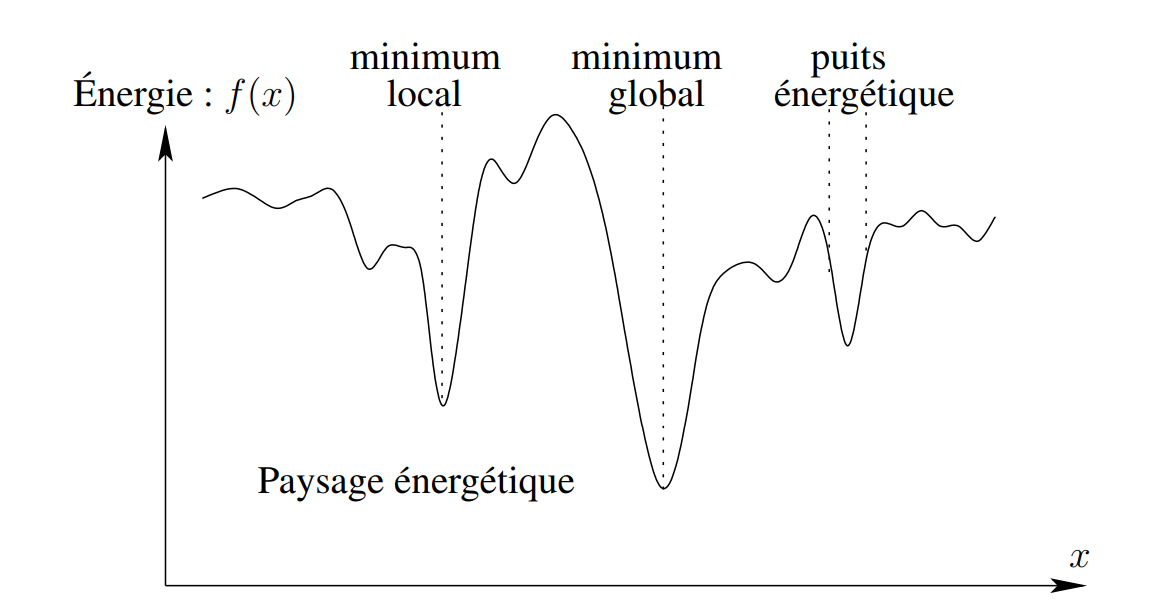
\includegraphics[height=2in]{img/Optimum_global_optimum_local.png}	
	\captionof{figure}{Paysage énergétique dans le cadre continu d’une fonction de coût pour un espace des
solutions à une dimension \citep{BICHOT2007}} \label{ogol}
\end{center}